%initialising document, adjust papersize, fontsize and page orientation to your needs
\documentclass[a4paper, fontsize = 8pt, landscape]{scrartcl}
\usepackage{../../../misc_files/LateX/layout_and_colours}
\title{Höhere Mathematik}
\author{Jil Zerndt, Lucien Perret}
\date{May 2024}

\createtitlepagestyle
\createmainpagestyle
\begin{document}
\begin{multicols}{3}
	\thispagestyle{TitlePageStyle}
	\maketitle
	%\section{Einführung SGMM und Umweltsphären}

\subsection{BWL Grundbegriffe}

\begin{definition}{BWL und Betrieb}\\
Die Betriebswirtschaftslehre ist eine Teilwissenschaft der Wirtschaftswissenschaften und beschäftigt sich mit der Analyse und Gestaltung von betrieblichen Entscheidungen und Prozessen.

Ein Unternehmen ist eine eigenständige, rechtliche und wirtschaftliche Einheit, die Sachgüter und Dienstleistungen anbietet. Der \textbf{Betrieb} ist die örtliche Produktionsstätte, während die \textbf{Firma} im rechtlichen Sinn der Name des Unternehmens ist.
\end{definition}

\begin{definition}{Ökonomisches Prinzip}\\
Das ökonomische Prinzip beschreibt das rationale wirtschaftliche Handeln und kann in drei Ausprägungen vorkommen:
\begin{itemize}
    \item \textbf{Minimalprinzip}: Mit gegebenen Mitteln maximalen Ertrag erzielen
    \item \textbf{Maximalprinzip}: Mit minimalen Mitteln einen vorgegebenen Ertrag erzielen
    \item \textbf{Optimumprinzip}: Mit möglichst wenig Aufwand einen möglichst hohen Ertrag erzielen
\end{itemize}
\end{definition}

\begin{definition}{Bedürfnis\, Bedarf und Nachfrage}\\
\begin{itemize}
    \item \textbf{Bedürfnis}: Empfundener Mangel und der Wunsch, diesen zu beseitigen
    \item \textbf{Bedarf}: Ökonomisch relevantes, durch Kaufkraft gedecktes Bedürfnis
    \item \textbf{Nachfrage}: Durch Kaufbereitschaft zum Ausdruck gebrachter Bedarf
\end{itemize}
\end{definition}

\begin{definition}{Güterarten}\\
Man unterscheidet verschiedene Arten von Gütern:
\begin{itemize}
    \item Nach Art: Sachgüter vs. Dienstleistungen
    \item Nach Verwendungszweck: Konsumgüter vs. Produktionsgüter
    \item Nach Knappheit: Freie Güter vs. wirtschaftliche Güter
    \item Nach Verfügbarkeit: Private Güter vs. öffentliche Güter
\end{itemize}
\end{definition}

\begin{definition}{Unternehmensverantwortung}\\
Die Unternehmensverantwortung umfasst drei Dimensionen:
\begin{itemize}
    \item \textbf{Ökonomische Verantwortung}: Profitabilität, Erhalt der Wettbewerbsfähigkeit
    \item \textbf{Ökologische Verantwortung}: Umweltschutz, nachhaltige Ressourcennutzung
    \item \textbf{Soziale Verantwortung}: Verantwortung gegenüber Mitarbeitern, Gesellschaft
\end{itemize}
Diese drei Dimensionen bilden das Prinzip der dreifachen Unternehmensverantwortung (Triple Bottom Line).
\end{definition}

\subsection{St. Galler Management-Modell (SGMM)}

\begin{concept}{SGMM als Managementmodell}\\
Das St. Galler Management-Modell (SGMM) dient als Denkgrundlage und Orientierungshilfe für praktische Fragestellungen im Unternehmenskontext. Es bietet:
\begin{itemize}
    \item Komplexitätsreduktion
    \item Ordnungsrahmen und Wirkungszusammenhänge
    \item Strukturierung der Kommunikation
    \item Gemeinsame Sprache für Managementfragen
\end{itemize}
\end{concept}

\begin{concept}{Kategorien des SGMM}\\
Das SGMM besteht aus folgenden Begriffskategorien:
\begin{itemize}
    \item Umweltsphären: Relevante Bezugsräume im Umfeld der Unternehmung
    \item Anspruchsgruppen: Gruppen und Individuen, die von der Unternehmenstätigkeit betroffen sind
    \item Interaktionsthemen: Gegenstände der Austauschbeziehungen zwischen Anspruchsgruppen und Unternehmen
    \item Ordnungsmomente: Strategie, Struktur, Kultur
    \item Entwicklungsmodi: Erneuerung und Optimierung
    \item Prozesse: Management-, Geschäfts- und Unterstützungsprozesse
\end{itemize}
\end{concept}

\subsection{Umweltsphären}

\begin{definition}{Umweltsphären}\\
Umweltsphären bezeichnen relevante Bezugsräume im Umfeld eines Unternehmens und beeinflussen dessen Handlungsspielraum. Man unterscheidet:
\begin{itemize}
    \item \textbf{Ökonomische Umwelt}: Wirtschaftliche Rahmenbedingungen, Arbeitsmarkt, Teuerung, internationale Wirtschaftsbeziehungen
    \item \textbf{Technologische Umwelt}: Technik und Naturwissenschaften, Produktionsverfahren, Materialien, Transport- und Kommunikationsmittel
    \item \textbf{Soziale Umwelt}: Gesellschaftliche Trends, Werte und Bedürfnisse der Menschen
    \item \textbf{Ökologische Umwelt}: Gesamthaushalt der Natur, Rohstoffe, Energie, Klima, Abfälle
\end{itemize}
\end{definition}

\subsection{Anspruchsgruppen}

\begin{definition}{Anspruchsgruppen (Stakeholder)}\\
Anspruchsgruppen (Stakeholder) sind alle Gruppen und Individuen, die in irgendeiner Form von der Tätigkeit eines Unternehmens betroffen sind. Zu den wichtigsten Anspruchsgruppen zählen:
\begin{itemize}
    \item Kapitalgeber (Eigenkapital- und Fremdkapitalgeber)
    \item Kunden
    \item Mitarbeitende
    \item Öffentlichkeit/NGOs
    \item Staat und Behörden
    \item Lieferanten
    \item Konkurrenz
\end{itemize}
Diese Anspruchsgruppen leiten aus ihrer Beziehung zum Unternehmen Erwartungen und Ansprüche ab, die sie selbst oder durch Interessenvertreter an das Unternehmen herantragen.
\end{definition}

\subsection{Interaktionsthemen}

\begin{definition}{Interaktionsthemen}\\
Interaktionsthemen sind Gegenstände der Austauschbeziehungen zwischen Anspruchsgruppen und dem Unternehmen. Man unterscheidet:
\begin{itemize}
    \item \textbf{Personen- und kulturgebundene Elemente}: Anliegen, Interessen, Normen und Werte
    \item \textbf{Objektgebundene Elemente}: Ressourcen (Kapital, Arbeit, Wissen, etc.)
\end{itemize}
\end{definition}

\begin{concept}{Interaktionsthemenanalyse}\\
Die Interaktionsthemenanalyse ist ein Instrument zur systematischen Untersuchung der Wechselbeziehungen zwischen einem Unternehmen und seinen Anspruchsgruppen. Dabei wird folgender Ablauf verfolgt:
\begin{itemize}
    \item \textbf{Schritt 1}: Beschreibung des Interaktionsthemas
    \begin{itemize}
        \item Welche Ressource des Unternehmens ist betroffen?
        \item In welcher Umweltsphäre spielt sich der Sachverhalt ab?
    \end{itemize}
    \item \textbf{Schritt 2}: Analyse der betroffenen Anspruchsgruppe
    \begin{itemize}
        \item Welche Anliegen bringt die Anspruchsgruppe vor?
        \item Welche Interessen verfolgt die Anspruchsgruppe?
        \item Welche Normen und Werte stützen die Anliegen?
    \end{itemize}
    \item \textbf{Schritt 3}: Bewertung aus Unternehmenssicht
    \begin{itemize}
        \item Welche Gefahren ergeben sich für das Unternehmen?
        \item Welche Reaktionsmöglichkeiten hat das Unternehmen?
    \end{itemize}
\end{itemize}
\end{concept}

\begin{example}
Eine Interaktionsthemenanalyse am Beispiel Tesla könnte so aussehen:
\begin{itemize}
    \item \textbf{Interaktionsthema}: Elektromobilität
    \item \textbf{Ressource}: Glaubwürdigkeit (Image) und Kapital
    \item \textbf{Umweltsphäre}: Natur/Umwelt
    \item \textbf{Anspruchsgruppe}: Kunden (Käufer von Tesla Automobilen)
    \item \textbf{Anliegen}: Umweltfreundliches Auto, "saubere" Mobilität
    \item \textbf{Interessen}: Wenig CO2-Ausstoss, Steuererleichterungen
    \item \textbf{Normen}: Umweltschutzgesetz, Verordnung über CO2-Emissionen, Subventionen
    \item \textbf{Werte}: Umweltschutz, Nachhaltigkeit
    \item \textbf{Gefahren aus Unternehmenssicht}: Verlust an Glaubwürdigkeit, Imageschaden, sinkende Verkaufszahlen durch Kürzung von Subventionszahlungen
    \item \textbf{Reaktionsmöglichkeiten}: Investitionen in F\&E bei der Batterieproduktion, Lobbying in der Politik, Imagekampagne
\end{itemize}
\end{example}

\subsection{Ordnungsmomente}

\begin{definition}{Ordnungsmomente}\\
Ordnungsmomente geben dem Alltagsgeschehen einer Unternehmung, das in Form von Prozessen abläuft, eine gesamtheitliche Ausrichtung und Sinngebung. Die drei Teilbereiche sind:
\begin{itemize}
    \item \textbf{Strategie}: Langfristige Ausrichtung und Ziele des Unternehmens
    \item \textbf{Struktur}: Aufbau- und Ablauforganisation des Unternehmens
    \item \textbf{Kultur}: Gemeinsame Werte, Normen und Überzeugungen
\end{itemize}
Zwischen Prozessen und Ordnungsmomenten besteht eine Wechselwirkung: Die Ordnungsmomente ergeben sich aus dem Alltagsgeschehen und strukturieren dieses wiederum.
\end{definition}

\subsection{Entwicklungsmodi}

\begin{definition}{Entwicklungsmodi}\\
Entwicklungsmodi bezeichnen die verschiedenen Arten der Weiterentwicklung einer Unternehmung:
\begin{itemize}
    \item \textbf{Optimierung}: Die kontinuierliche, ständig ablaufende Verbesserung des Bestehenden (inkrementelle Veränderung)
    \item \textbf{Erneuerung}: Die diskontinuierliche, nur sprunghaft stattfindende Schaffung von völlig Neuem (radikale Veränderung)
\end{itemize}
\end{definition}

\subsection{Prozesse}

\begin{definition}{Prozesse}\\
Das SGMM begreift eine Unternehmung als ein System von Prozessen, d.h. routinemässigen Abläufen, welche den unternehmerischen Alltag prägen. Je besser diese Abläufe optimiert sind, desto grösser ist in der Regel der Erfolg der Unternehmung. Man unterscheidet:
\begin{itemize}
    \item \textbf{Managementprozesse}: Grundlegende Aufgaben, die mit der Gestaltung, Lenkung und Entwicklung der Unternehmung zu tun haben (normative Orientierungsprozesse, strategische Entwicklungsprozesse und operative Führungsprozesse)
    \item \textbf{Geschäftsprozesse}: Kernaktivitäten einer Unternehmung, die auf den Kundennutzen ausgerichtet sind (Leistungserstellung, Vertrieb etc.)
    \item \textbf{Unterstützungsprozesse}: Interne Dienstleistungen für einen effektiven Vollzug der Geschäftsprozesse (Personal, EDV, Finanzen etc.)
\end{itemize}
\end{definition}
	\section{Rechnerarithmetik}

\subsection{Zahlendarstellung und Maschinenzahlen}

Maschinendarstellbare Zahlen $M$ zur Basis $B$ :

$$
M=\left\{x \in \mathbb{R} \mid x= \pm 0 . m_{1} m_{2} m_{3} \ldots m_{n} \cdot B^{ \pm e_{1} e_{2} \ldots e_{l}}\right\} \cup\{0\}
$$

Dabei gilt $m_{1} \neq 0, m_{i}, e_{i} \in\{0,1, \ldots, B-1\}$ für $i \neq 0$ und $B \in \mathbb{N}(B>1)$

\section*{Der Wert $\widehat{\boldsymbol{\omega}}$ einer solchen Zahl ist definiert als}
$$
\widehat{\omega}=\sum_{i=1}^{n} m_{i} B^{\hat{\mathrm{e}}-i}, \quad \hat{\mathrm{e}}=\sum_{l=1}^{l} e_{i} B^{l-i}
$$

$x$ wird als n -stellige Gleitpunktzahl zur Basis $B$ bezeichnet.\\
Beispiel: $\underbrace{0.3211}_{n=4} \cdot \underbrace{4^{12}}_{l=2}$

\begin{enumerate}
  \item $\hat{e}=1 \cdot 4^{1}+2 \cdot 4^{0}=6$
  \item $\widehat{\omega}=3 \cdot 4^{5}+2 \cdot 4^{4}+1 \cdot 4^{3}+1 \cdot 4^{2}=3664$
\end{enumerate}

\section*{Gleitpunktzahlen}
\begin{itemize}
  \item Single Precision (32 Bit) $\quad V=1$ Bit $\quad E=8$ Bit $\quad M=23$ Bit
  \item Double Precision (64 Bit) $V=1$ Bit $\quad E=11$ Bit $\quad M=52$ Bit
\end{itemize}

Bei allgemeiner Basis $B$ gilt (Maschinengenauigkeit $=e p s$ )

$$
\text { eps }:=\frac{B}{2} \cdot B^{-n}, \quad e p s_{10}:=5 \cdot 10^{-n}
$$

Sie bezeichnet den maximalen relativen Fehler, der durch Rundungen entstehen kann.

$$
\left|\frac{r d(x)-x}{x}\right| \leq 5 \cdot 10^{-n} \quad\left(\text { da } x \geq 10^{e-1}\right)
$$

\subsection{Approximations- und Rundungsfehler}

Die Maschinenzahlen sind nicht gleichmässig verteilt. Bei jedem Rechner gibt es eine grösste $\left(x_{\max }\right)$ und kleinste $\left(x_{\min }\right)$ positive Maschinenzahl.

\begin{itemize}
  \item $x_{\text {max }}=B^{e_{\max }}-B^{e_{\max }-n}=\left(1-B^{-n}\right) \cdot B^{e_{\max }}$
  \item $x_{\text {min }}=B^{e_{\text {min }}-1}$
\end{itemize}

\section*{Definition}
Gegeben sei eine Näherung $\tilde{x}$ zu einem exakten Wert $x$

\begin{itemize}
  \item Absoluter Fehler\\
$|\tilde{x}-x|$
  \item Relativer Fehler\\
$\left|\frac{\tilde{x}-x}{x}\right| b z w \cdot \frac{|\tilde{x}-x|}{|x|}$
\end{itemize}

\section*{Fehlerfortpflanzung bei Funktionsauswertungen / Konditionierung}
Näherung für den absoluten und relativen Fehler bei Funktionsauswertungen

$$
\begin{aligned}
\underbrace{|f(\tilde{x})-f(x)|}_{\text {absoluter Fehler von } f(x)} & \approx\left|f^{\prime}(x)\right| \cdot \underbrace{|\tilde{x}-x|}_{\text {absoluter Fehler von } x} \\
\underbrace{\frac{|f(\tilde{x})-f(x)|}{|f(x)|}}_{\text {relativer Fehler von } f(x)} & \approx \underbrace{\frac{\left|f^{\prime}(x)\right| \cdot|x|}{|f(x)|}}_{\text {Konditionszahl } K} . \quad \underbrace{|\tilde{x}-x|}_{\begin{array}{c}
|x| \\
\text { relativer Fehler von } x
\end{array}}
\end{aligned}
$$

Den Faktor $K$ nennt man Konditionszahl.

$$
K:=\frac{\left|f^{\prime}(x)\right| \cdot|x|}{|f(x)|}
$$

Relative Fehlervergrösserung von $x$, bei einer Funktionsauswertung von $f(x)$.

\begin{center}
\begin{tabular}{ll}
- Gut konditionierte Probleme & Konditionszahl ist klein $(\leq 1)$ \\
- Schlecht konditionierte Probleme & Konditionszahl ist gross $(>1)$ \\
\end{tabular}
\end{center}
	\section{Lösung von Nullstellenproblemen}

\subsection{Problemstellung NSP}

Eine Gleichung der Form $F(x)=x$ heisst Fixpunktgleichung.

\begin{itemize}
  \item Ihre Lösungen $\bar{x}$, für die $F(\bar{x})=\bar{x}$ erfüllt ist, heissen Fixpunkte.
\end{itemize}

\subsection{Fixpunktiteration}

Gegeben sei $F:[a, b] \rightarrow \mathbb{R}$, mit $x_{0} \in[a, b]$. Die rekursive Folge

$$
x_{x+1} \equiv F\left(x_{n}\right), \quad n=0,1,2, \ldots
$$

Heisst Fixpunktiteration von $F$ zum Startwert $x_{0}$.\\
Sei $F:[a, b] \rightarrow \mathbb{R}$ mit stetiger Ableitung $F^{\prime}$ und $\bar{x} \in[a, b]$ ein Fixpunkt von $F$. Dann gilt für die Fixpunktiteration $x_{n+1}=F\left(x_{n}\right)$

\begin{itemize}
  \item $\quad\left|F^{\prime}(\bar{x})\right|<1 \quad x_{n}$ konvergiert gegen $\bar{x}$, falls $x_{0}$ nahe genug bei $\bar{x}$ liegt anziehend
  \item $\left|F^{\prime}(\bar{x})\right|>1 \quad x_{n}$ konvergiert für keinen Startwert $x_{0} \neq \bar{x}$ abstossend
\end{itemize}

\section*{Banachscher Fixpunktsatz}
Sei $F:[a, b] \rightarrow[a, b]$ und es existiere eine Konstante $\alpha$, wobei gilt

\begin{itemize}
  \item $\alpha(0<\alpha<1)$ : Lipschitz-Konstante
  \item $\forall_{x, y}(x, y \in[a, b])$
\end{itemize}

$$
|F(x)-F(y)| \leq \alpha|x-y|, \quad \frac{|F(x)-F(y)|}{|x-y|} \leq \alpha
$$

Dann gilt

\begin{itemize}
  \item $\quad F$ hat genau einen Fixpunkt $\bar{x}$ in $[a, b]$
  \item Die Fixpunktiteration $x_{n+1}=F\left(x_{n}\right)$ konvergiert gegen $\bar{x}$ für alle Startwerte $x_{0} \in[a, b]$
  \item Es gelten die Fehlerabschätzungen
  \item $\left|x_{n}-\bar{x}\right| \leq \frac{\alpha^{n}}{1-\alpha} \cdot\left|x_{1}-x_{0}\right| \quad$ a-priori Abschätzung
  \item $\left|x_{n}-\bar{x}\right| \leq \frac{\alpha}{1-\alpha} \cdot\left|x_{n}-x_{n-1}\right| \quad$ a-posteriori Abschätzung
\end{itemize}

Berechne die Nullstellen von $p(x)=x^{3}-x+0.3$\\
Fixpunktiteration

$$
x_{n+1}=F\left(x_{n}\right)=x_{n}^{3}+0.3
$$

$F\left(x_{n}\right)$ steigt stetig an\\
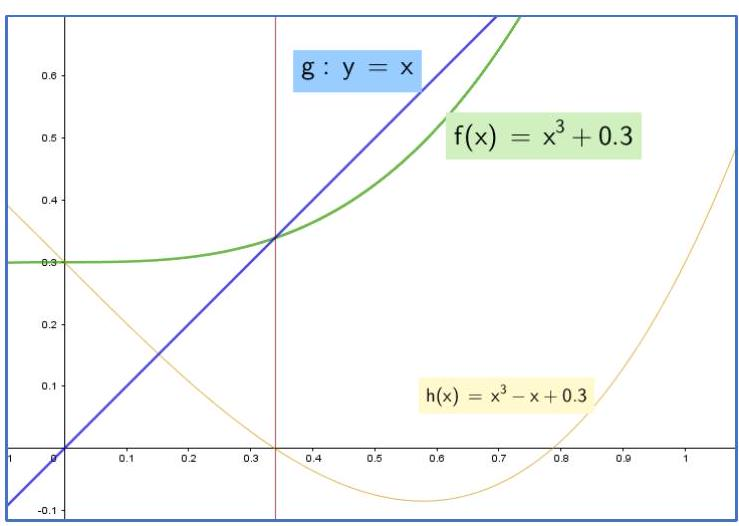
\includegraphics[width=\linewidth]{images/2024_12_29_68ccba06d0091c162fa4g-02}\\
$F: I \rightarrow I$ gilt wenn...

$$
F(a)>a, \quad F(b)<b
$$

Alpha bestimmen / überprüfen

$$
\alpha=\max _{x \in I}\left|F^{\prime}(x)\right| \leq 1
$$

Anzahl Iterationen $n$ berechnen

$$
n \geq \frac{\ln \left(\frac{t o l \cdot(1-\alpha)}{\left|x_{1}-x_{0}\right|}\right)}{\ln \alpha}
$$

\subsection{Newton-Verfahren}

Sukzessive Approximation der Funktionskurve $y=f(x)$ durch Tangenten, deren Schnittpunkt mit der x-Achse problemlos berechnet werden kann

Lösung $\xi$ der Gleichung $f(x)=0$ finden.\\
$>$ Startwert $x_{0}$ geeignet wählen (nahe bei $\xi$ )\\
$>$ Iterationsvorschrift:

$$
x_{n+1}=x_{n}-\frac{f\left(x_{n}\right)}{f^{\prime}\left(x_{n}\right)}
$$

Die Folge $\left(x_{n}\right)_{n \in \mathbb{N}}$ konvergiert gegen die Lösung $\xi$ der Gleichung $f(x)=0$.\\
$\left(x_{0}, x_{1}, x_{2}, \ldots\right)$ ist sicher gegeben, wenn im Intervall $[a, b]$, in dem alle Näherungswerte (und die Nullstellen selbst) liegen sollen, die Bedingung

$$
\left|\frac{f(x) \cdot f^{\prime \prime}(x)}{\left[f^{\prime}(x)\right]^{2}}\right|<1
$$

Erfüllt ist (hinreichende Konvergenzbedingung).

\section*{Vereinfachtes Newton-Verfahren}
Statt in jedem Schritt $f^{\prime}\left(x_{n}\right)$ auszurechnen, kann man immer wieder $f^{\prime}\left(x_{0}\right)$ verwenden.

$$
x_{n+1}=x_{n}-\frac{f\left(x_{n}\right)}{f^{\prime}\left(x_{0}\right)}
$$

\section*{Sekantenverfahren}
Der Schnittpunkt von Sekanten durch jeweils zwei Punkte $\left(x_{0}, f\left(x_{0}\right)\right)$ und $\left(x_{1}, f\left(x_{1}\right)\right)$ mit der $x$-Achse, wird berechnet.

$$
x_{n+1}=x_{n}-\frac{x_{n}-x_{n-1}}{f\left(x_{n}\right)-f\left(x_{n-1}\right)} \cdot f\left(x_{n}\right)
$$

\subsection{Konvergenzgeschwindigkeit}

Sei $\left(x_{n}\right)$ eine gegen $\bar{x}$ konvergierende Folge. Dann hat das Verfahren die Konvergenzordnung $q \geq 1$ wenn es eine Konstante $c>0$ gibt mit

$$
\left|x_{n+1}-\bar{x}\right| \leq c \cdot\left|x_{n}-\bar{x}\right|^{q}
$$

Für alle $n$.

\begin{itemize}
  \item $q=1 \quad$ lineare Konvergenz $\quad$ verlangt man noch $c<1$.
  \item $q=2$ quadratische Konvergenz
\end{itemize}

\subsection{Fehlerabschätzung}

Nullstellensatz von Bolzano\\
Sei $f:[a, b] \rightarrow \mathbb{R}$ stetig mit $f(a) \leq 0 \leq f(b)$ oder $f(a) \geq 0 \geq f(b)$. Dann muss $f$ in $[a, b]$ eine Nullstelle besitzen.

Sei $x_{n}$ also ein iterativ bestimmter Näherungswert einer exakten Nullstelle $\xi$ der stetigen Funktion $F: \mathbb{R} \rightarrow \mathbb{R}$ und es gelte für ein vorgegebene Fehlerschranke / Fehlertolerant $\epsilon>0$

$$
f\left(x_{n}-\epsilon\right) \cdot f\left(x_{n}+\epsilon\right)<0
$$

Dann muss gemäss dem Nullstellensatz im offenen Intervall $\left(x_{n}-\epsilon, x_{n}+\epsilon\right)$ eine Nullstelle $\xi$ liegen und es gilt die Fehlerabschätzung

$$
\left|x_{n}-\xi\right|<\epsilon
$$
	\section{Lineare Gleichungssysteme}

\subsection{Gauss-Algorithmus}

Gauss-Algorithmus für ein Gleichungssystem $A x=b$ :

$$
A=\left[\begin{array}{ccc}
a_{11} & \cdots & a_{1 n} \\
\vdots & \ddots & \vdots \\
a_{n 1} & \cdots & a_{n n}
\end{array}\right] \in \mathbb{R}^{n \times n}, \quad x=\left(\begin{array}{c}
x_{1} \\
\vdots \\
x_{n}
\end{array}\right) \in \mathbb{R}^{n}, \quad b=\left(\begin{array}{c}
b_{1} \\
\vdots \\
b_{n}
\end{array}\right) \in \mathbb{R}^{n}
$$

Umformung des Gleichungssystems $A x=b$, in ein äquivalentes Gleichungssystem $\tilde{A} x=b$, so dass die Matrix $\tilde{A}$ als obere Dreiecksmatrix vorliegt.

\begin{itemize}
  \item $\quad z_{j}:=z_{j}-\lambda z_{i} \quad i<j(\lambda \in \mathbb{R}), z_{i}$ ist die $i$-te Zeile des Gleichungssystems
  \item $\quad z_{i} \rightarrow z_{j} \quad$ Vertauschen der $i$-ten und $j$-ten Zeile im System
\end{itemize}

Rekursive Vorschrift für ein Gleichungssystem $\tilde{A} x=b$ :

$$
\begin{gathered}
x_{n}=\frac{b_{n}}{a_{n n}}, x_{n-1}=\frac{b_{n-1}-a_{(n-1) n} \cdot x_{n}}{a_{n-1 n-1}}, \ldots, x_{1}=\frac{b_{1}-a_{12} \cdot x_{2}-\cdots-a_{1 n} \cdot x_{n}}{a_{11}} \\
x_{i}=\frac{b_{i}-\sum_{j=i+1}^{n} a_{i j} \cdot x_{j}}{a_{i i}}, \quad i=n, n-1, \ldots, 1
\end{gathered}
$$

\subsection{Fehlerfortpflanzung und Pivotisierung}

Für $i=1, . . n$ :\\
Erzeuge Nullen unterhalb des Diagonalelements in der i-ten Spalte

\begin{itemize}
  \item Suche das betragsgrösste Element unterhalb der Diagonalen in der i-ten Spalte: Wähle $k$ so, dass $\left|a_{k i}\right|=\max \left\{\left|a_{j i}\right| \mid j=i, \ldots n\right\}$
\end{itemize}

$$
\left\{\begin{array}{l}
\text { falls } a_{k i}=0: \quad \text { A ist nicht regulär; stop; } \\
\text { falls } a_{k i} \neq 0: \quad z_{k} \leftrightarrow z_{i}
\end{array}\right.
$$

\begin{itemize}
  \item Eliminationsschritt:
\end{itemize}

Für $j=i+1, \ldots, n$ eliminiere das Element $a_{j i}$ durch

$$
z_{j}:=z_{j}-\frac{a_{j i}}{a_{i i}} \cdot z_{i}
$$

\subsection{Dreieckszerlegung von Matrizen}

\subsubsection{Determinante}

Gegeben sei eine Matrix $A$, woraus die obere Dreiecksmatrix $\tilde{A}$ entsteht.

\begin{itemize}
  \item $\quad \tilde{a}_{i i}: \quad$ Diagonalelemente von $\tilde{A}$
  \item $\quad l: \quad$ Anzahl Zeilenvertauschungen
\end{itemize}

$$
\operatorname{det}(A)=(-1)^{l} \cdot \operatorname{det}(\tilde{A})=(-1)^{l} \cdot \prod_{i=1}^{n} \tilde{a}_{i i}
$$

Beispiel

$$
\begin{aligned}
\left(\begin{array}{ccc}
3 & 5 & 1 \\
0 & 2 & 2 \\
6 & 14 & 8
\end{array}\right) & =\left(\begin{array}{lll}
3 & 5 & 1 \\
0 & 2 & 2 \\
0 & 4 & 6
\end{array}\right)=\left(\begin{array}{lll}
3 & 5 & 1 \\
0 & 2 & 2 \\
0 & 0 & 2
\end{array}\right) \\
\operatorname{det}(A) & =(3) \cdot(2) \cdot(2)=12
\end{aligned}
$$

\subsubsection{LR-Zerlegung}

Das ursprüngliche Gleichungssystem $\boldsymbol{A} \boldsymbol{x}=\boldsymbol{b}$ lautet mit der $L R$-Zerlegung

$$
L R x=b \Leftrightarrow L y=b \text { und } R x=y
$$

Für eine $n \times n$ Matrix $A$, gibt es $n \times n$ Matrizen $L$ und $R$ mit den Eigenschaften

\begin{itemize}
  \item $L$ ist eine normierte untere Dreiecksmatrix $\operatorname{mit} l_{i i}=1(i=1, \ldots, n)$
  \item $R$ ist eine obere Dreiecksmatrix\\
$\operatorname{mit} r_{i i} \neq 0(i=1, \ldots, n)$
  \item $\quad A=L \cdot R$ ist die $L R$-Zerlegung von $A$.
\end{itemize}

\section*{Zerlegung mit Zeilenvertauschung}
$P_{K}$ erhält man aus der Einheitsmatrix $I_{n}$ durch Vertauschen der $i$-ten und $j$-ten Zeile.\\
Zeilen-Vertauschungen werden durch $P_{1} \ldots P_{n}$ ausgedrückt.

$$
P=\prod_{i=1}^{n} P_{n-i+1}
$$

Mit dieser Permutationsmatrix erhält man dann als $R L-$ Zerlegung

$$
P A=L R
$$

Das lineare Gleichungssystem $A x=b$ lässt sich schreiben als $P A x=P b$ bzw. $L R x=$ $P b$ und in den zwei Schritten lösen

$$
\begin{gathered}
L y=P b \rightarrow y=\cdots \\
R x=y \rightarrow x=\cdots
\end{gathered}
$$

Vertauschung der 1. Und 3. Zeile bei der Matrix

$$
\begin{gathered}
A=\left(\begin{array}{lll}
1 & 2 & 3 \\
4 & 5 & 6 \\
7 & 8 & 9
\end{array}\right) \rightarrow A^{*}=\left(\begin{array}{lll}
7 & 8 & 9 \\
4 & 5 & 6 \\
1 & 2 & 3
\end{array}\right) \\
I^{*} \cdot A=P_{1} \cdot A=A^{*}=\left(\begin{array}{lll}
0 & 0 & 1 \\
0 & 1 & 0 \\
1 & 0 & 0
\end{array}\right)\left(\begin{array}{lll}
1 & 2 & 3 \\
4 & 5 & 6 \\
7 & 8 & 9
\end{array}\right)=\left(\begin{array}{lll}
7 & 8 & 9 \\
4 & 5 & 6 \\
1 & 2 & 3
\end{array}\right) \\
A=\left(\begin{array}{ccc}
-1 & 1 & 1 \\
1 & -3 & -2 \\
5 & 1 & 4
\end{array}\right)=L R \\
i=1, j=2 \rightarrow z_{2}=z_{2}-\frac{1}{(-1)} \cdot z_{1} \rightarrow A_{1}=\left(\begin{array}{ccc}
-1 \\
1-1 & -3+1 & -1+1 \\
5 & 1 & 4
\end{array}\right) \\
i=1, j=3 \rightarrow z_{3}=z_{3}-\underbrace{\frac{5}{(-1)}}_{l_{21}} \cdot z_{1} \rightarrow A_{2}=\left(\begin{array}{ccc}
-1 & 1 & 1 \\
0 & -2 & -1 \\
5-5 & 1+5 & 4+5
\end{array}\right) \\
i=2, j=3 \rightarrow z_{3} \equiv z_{3}-\underbrace{\frac{6}{(-2)}}_{l_{32}} \cdot z_{2} \rightarrow A_{3}=\left(\begin{array}{c}
-1 \\
0 \\
0+0 \\
0
\end{array}\right. \\
R=2
\end{gathered}
$$

Einsetzen in $L$

$$
\begin{gathered}
l_{21}=\frac{1}{-1}=-1, \quad l_{31}=\frac{5}{-1}=-5, \quad l_{32}=\frac{6}{-2}=-3 \\
L=\left(\begin{array}{ccc}
1 & 0 & 0 \\
l_{21} & 1 & 0 \\
l_{31} & l_{32} & 1
\end{array}\right)=\left(\begin{array}{ccc}
1 & 0 & 0 \\
-1 & 1 & 0 \\
5 & -3 & 1
\end{array}\right)
\end{gathered}
$$

\subsubsection{QR-Zerlegung}

Eine Matrix $Q \in \mathbb{R}^{n \times n}$ heisst orthogonal, wenn $Q^{T} \cdot Q=I_{n}$ ist. Dabei ist $I_{n}$ die $n \times n$ Einheitsmatrix.

Sei $A \in \mathbb{R}^{n \times n}$. Eine $Q R$-Zerlegung von $A$ ist eine Darstellung von $A$ als Produkt einer orthogonalen $n \times n$ Matrix $Q$ und einer rechtsoberen $n \times n$ Dreiecksmatrix $R$

$$
A=Q R
$$

Lösung des Gleichungssystems

$$
A x=b \Leftrightarrow Q R x=b \Leftrightarrow R x=Q^{T} b
$$

Algorithmus zur QR-Zerlegung

$$
R:=A, \quad Q:=I_{n}
$$

Für $i=1, \ldots, n-1$ :\\
erzeuge Nullen in $R$ in der $i$-ten Spalte unterhalb der Diagonalen

\begin{enumerate}
  \item $H_{i}$ mit $(n-i+1) \times(n-i+1)$ berechnen
  \item $H_{i}$ mit $I_{i-1}$ Block links oben erweitern $\rightarrow Q_{i}$
  \item $R:=Q_{i} \cdot R$
  \item $Q:=Q \cdot Q_{i}^{T}$
\end{enumerate}

Ablauf

$$
\begin{gathered}
H_{1} \cdot A_{1}=H_{1} \cdot \underbrace{\left(\begin{array}{lll}
* & * & * \\
* & * & * \\
* & * & *
\end{array}\right)}_{A_{1}}=\left(\begin{array}{lll}
* & * & * \\
0 & * & * \\
0 & * & *
\end{array}\right) \rightarrow \underbrace{\left(\begin{array}{cc}
* & * \\
* & *
\end{array}\right)}_{A_{2}} \\
a_{1}=\left(\begin{array}{l}
a_{11} \\
a_{21} \\
a_{31}
\end{array}\right), \quad e_{1}=\left(\begin{array}{l}
1 \\
0 \\
0
\end{array}\right)
\end{gathered}
$$

\begin{enumerate}
  \item $v_{1}:=a_{1}+\operatorname{sign}\left(a_{11}\right) \cdot\left|a_{1}\right| \cdot e_{1}$
  \item $u_{1}:=\frac{1}{\left|v_{1}\right|} \cdot v_{1}$
  \item $H_{1}:=I_{n}-2 u_{1} u_{1}^{T}=Q_{1}$
\end{enumerate}

$$
\begin{gathered}
H_{2} \cdot A_{2}=H_{2} \cdot \underbrace{\left(\begin{array}{ll}
* & * \\
* & *
\end{array}\right)}_{A_{2}}=\left(\begin{array}{ll}
* & * \\
0 & *
\end{array}\right) \\
Q_{2}=\left(\begin{array}{ccc}
1 & 0 & 0 \\
0 & H_{2} & H_{2} \\
0 & H_{2} & H_{2}
\end{array}\right)
\end{gathered}
$$

$$
Q:=Q_{1}^{T} \cdot Q_{2}^{T}, \quad R:=\underbrace{Q_{2} \cdot Q_{1}}_{Q^{-1}} \cdot A
$$

\subsection{Fehlerrechnung und Aufwandabschätzung}

Eine Abbildung $\|\|:. \mathbb{R}^{n} \rightarrow \mathbb{R}$ heisst Vektornorm, wenn die folgenden Bedingungen für alle $x, y \in \mathbb{R}^{n}, \lambda \in \mathbb{R}$ erfüllt sind:

\begin{itemize}
  \item $\|x\| \geq 0$ und $\|x\|=0 \Leftrightarrow x=0$
  \item $\|\lambda x\|=|\lambda| \cdot\|x\|$
  \item $\|x+y\| \leq\|x\|+\|y\|$ "Dreiecksgleichung"
\end{itemize}

Für Vektoren $x=\left(x_{1}, x_{2}, \ldots, x_{n}\right)^{T} \in \mathbb{R}^{n}$ gibt es die folgenden Vektornormen

\begin{itemize}
  \item 1-Norm Summennorm
\end{itemize}

$$
\begin{aligned}
& \|x\|_{1}=\sum_{i=1}^{n}\left|x_{i}\right| \\
& \|x\|_{2}=\sqrt{\sum_{i=1}^{n} x_{i}^{2}} \\
& \|x\|_{\infty}=\max _{i=1, \ldots, n}\left|x_{i}\right|
\end{aligned}
$$

\begin{itemize}
  \item 2-Norm Euklidische Norm
  \item $\infty$-Norm Maximumnorm
\end{itemize}

Für eine $n \times n$ Matrix $A \in \mathbb{R}^{n \times n}$ gibt es die folgenden Matrixnormen

\begin{itemize}
  \item 1-Norm Spaltensummennorm $\|A\|_{1}=\max _{j-1, \ldots, n} \sum_{i=1}^{n}\left|x_{i}\right|$
  \item 2-Norm Spektralnorm $\quad\|A\|_{2}=\sqrt{\rho\left(A^{T} A\right)}$
  \item $\infty$-Norm Zeilensummennorm $\|A\|_{\infty}=\max _{i=1, \ldots, n} \sum_{j=1}^{n}\left|a_{i j}\right|$
\end{itemize}

\subsubsection{Fehlerabschätzung}

\paragraph{Abschätzung für Fehlerhafte Matrizen}
Sei $\|$.$\| eine Norm, A, \tilde{A} \in \mathbb{R}^{n \times n}$ eine reguläre $n \times n$ Matrix und $x, \tilde{x}, b, \tilde{b} \in$ $\mathbb{R}^{n}$ mit $A x=b$ und $\tilde{A} \tilde{x}=\tilde{b}$. Falls

$$
\operatorname{cond}(A) \cdot \frac{\|A-\tilde{A}\|}{\|A\|}<1
$$

Dann gilt

$$
\frac{\|x-\tilde{x}\|}{\|x\|} \leq \frac{\operatorname{cond}(A)}{1-\operatorname{cond}(A) \cdot \frac{\|A-\tilde{A}\|}{\|A\|}} \cdot\left(\frac{\|A-\tilde{A}\|}{\|A\|}+\frac{\|b-\tilde{b}\|}{\|b\|}\right)
$$

\paragraph{Abschätzung für Fehlerhafte Vektoren}
Sei $\|$. $\|$ eine Norm, $A \in \mathbb{R}^{n \times n}$ eine reguläre $n \times n$ Matrix und $x, \tilde{x}, b, \tilde{b} \in \mathbb{R}^{n}$ mit $A x=b$ und $A \tilde{x}=\tilde{b}$. Dann gilt für den absoluten und den relativen Fehler in $x$ :

\begin{itemize}
  \item $\|x-\tilde{x}\| \leq\left\|A^{-1}\right\| \cdot\|b-\tilde{b}\|$
  \item $\frac{\|x-\tilde{x}\|}{\|x\|} \leq\|A\| \cdot\left\|A^{-1}\right\| \cdot \frac{\|b-\tilde{b}\|}{\|b\|}$, falls $\|b\| \neq 0$\\
$\operatorname{Die}$ Zahl cond $(A)=\|A\| \cdot\left\|A^{-1}\right\|$ nennt man Konditionszahl der Matrix $A$
  \item $\quad \operatorname{cond}(A)$ gross $\rightarrow$ schlechte Konditionierung
\end{itemize}

Untersuchen Sie die Fehlerfortpflanzung im linearen Gleichungssystem $A x=b$ mit

$$
A=\left(\begin{array}{cc}
2 & 4 \\
4 & 8.1
\end{array}\right), \quad b=\binom{1}{1.5}
$$

Für den Fall, dass die rechte Seite von $\tilde{b}$ in jeder Komponente um maximal 0.1 von $b$ abweicht.

$$
\begin{gathered}
\|\tilde{b}-b\|_{\infty} \leq 0.1, \quad\|A\|_{\infty}=\max \{2+4,4+8.1\}=12.1 \\
\left\|A^{-1}\right\|_{\infty}=\left\|\left(\begin{array}{cc}
40.5 & -20 \\
-20 & 10
\end{array}\right)\right\|_{\infty}=60.5 \\
\operatorname{cond}(A)_{\infty}=\|A\|_{\infty} \cdot\left\|A^{-1}\right\|_{\infty}=12.1 \cdot 60.5=732.05 \\
\|x-\tilde{x}\|_{\infty} \leq\left\|A^{-1}\right\|_{\infty} \cdot\|b-\tilde{b}\|_{\infty} \leq 60.5 \cdot 0.1=\underbrace{6.05}_{\text {absoluter Fehler }} \\
\frac{\|x-\tilde{x}\|_{\infty}}{\|x\|_{\infty}} \leq \operatorname{cond}(A)_{\infty} \cdot \frac{\|b-\tilde{b}\|_{\infty}}{\|b\|_{\infty}} \leq 732 \cdot \frac{0.1}{1.5}=\underbrace{48.8}_{\text {relativer Fehler }}
\end{gathered}
$$

\subsubsection{Aufwandabschätzung}

Die Anzahl Gleitkommaoperationen werden in Abhängigkeit von $n$ bestimmt.

$$
\sum_{i=1}^{n} i=\frac{(n+1) \cdot n}{2} \text { und } \sum_{i=1}^{n} i^{2}=\frac{1}{3} n^{3}+\frac{1}{2} n^{2}+\frac{1}{6} n, \quad n=\text { Dimension }
$$

Ein Algorithmus hat die Ordnung $O\left(n^{q}\right)$, wenn $q>0$ die minimale Zahl ist, für die es eine Konstante $C>0$ gibt, so dass der Algorithmus für alle $n \in N$ weniger als

\section*{Beispiel}
Wie viele Gleitkommaoperationen benötigt das Rückwärtseinsetzen gemäss Gauss?

$$
x_{i}=\frac{b_{i}-\sum_{j=i+1}^{n} a_{i j} \cdot x_{j}}{a_{i i}}, \quad i=n, n-1, \ldots, 1
$$

Multiplikation und Division

$$
1+2+3+\cdots+n=\sum_{i=1}^{n} i=\frac{(n+1) \cdot n}{2}
$$

Addition und Subtraktion

$$
0+1+2+\cdots+n-1=\sum_{i=1}^{n-1} i=\frac{(n-1+1) \cdot(n-1)}{2}=\frac{(n-1) \cdot n}{2}
$$

Summe beider Operationstypen

$$
\frac{n^{2}}{2}+\frac{n}{2}+\frac{n^{2}}{2}-\frac{n}{2}=n^{2}
$$

\subsection{Iterative Verfahren}

Iterative Verfahren sind effizienter, jedoch kann man keine genauen Lösungen erwarten. Ausgehend von einem Startvektor $x^{(0)}$ berechnet man mittels einer Rechenvorschrift $F: \mathbb{R}^{n} \rightarrow \mathbb{R}^{n}$ iterativ eine Folge von Vektoren

$$
x^{(k+1)}=F\left(x^{(k)}\right) \text { mit } k=0,1,2, \ldots
$$

Zu lösen sei $A x=b$. Die Matrix $A=\left(a_{i j}\right)$ sei zerlegt in der Form $A=L+D+R=$

\subsubsection{Jacobi-Verfahren}

$$
\begin{gathered}
A x=b, \quad A=\left(\begin{array}{lll}
8 & 5 & 2 \\
5 & 9 & 1 \\
4 & 2 & 7
\end{array}\right), \quad b=\left(\begin{array}{c}
19 \\
5 \\
34
\end{array}\right), \quad x^{(0)}=\left(\begin{array}{c}
1 \\
-1 \\
3
\end{array}\right) \\
x_{1}^{(1)}=\frac{1}{8}\left(19-\sum_{j=1, j \neq 1}^{3} a_{1 j} \cdot x_{j}^{(0)}\right)=\frac{1}{8}(19-(5 \cdot-1+2 \cdot 3))=\frac{18}{8} \\
x_{2}^{(1)}=\frac{1}{9}\left(5-\sum_{j=1, j \neq 2}^{3} a_{2 j} \cdot x_{j}^{(0)}\right)=\frac{1}{9}(5-(5 \cdot 1+1 \cdot 3))=-\frac{1}{3} \\
x_{3}^{(1)}=\frac{1}{7}\left(34-\sum_{j=1, j \neq 3}^{3} a_{3 j} \cdot x_{j}^{(0)}\right)=\frac{1}{7}(34-(4 \cdot 1+2 \cdot-1))=\frac{32}{7}
\end{gathered}
$$

Fixpunktiteration gemäss Jacobi (Gesamtschritt-Verfahren):

$$
\begin{aligned}
& D x^{(k+1)}=-(L+R) x^{(k)}+b \\
& x^{(k+1)}=-D^{-1}(L+R) x^{(k)}+D^{-1} b
\end{aligned}
$$

Implementation /Allgemeine Form gemäss Jacobi

$$
x_{i}^{(k+1)}=\frac{1}{a_{i i}}\left(b_{i}-\sum_{j=1, j \neq i}^{n} a_{i j} \cdot x_{j}^{(k)}\right), \quad i=1, \ldots, n
$$

\subsubsection{Gauss-Seidel-Verfahren}

Fixpunktiteration gemäss Gauss-Seidel (Einzelschritt-Verfahren):

$$
\begin{aligned}
& (D+L) x^{(k+1)}=-R x^{(k)}+b \\
& x^{(k+1)}=-(D+L)^{-1} \cdot R x^{(k)}+(D+L)^{-1} \cdot b
\end{aligned}
$$

Implementation / Allgemeine Form gemäss Gauss-Seidel\\
$x_{i}^{(k+1)}=\frac{1}{a_{i i}}\left(b_{i}-\sum_{j=1}^{i-1} a_{i j} \cdot x_{j}^{(k+1)}-\sum_{j=i+1}^{n} a_{i j} \cdot x_{j}^{(k)}\right), \quad i=1, \ldots, n$

\subsubsection{Konvergenz der Fixpunktiteration}

Gegeben sei eine Fixpunktiteration

$$
x^{(n+1)}=B x^{(n)}+c=: F\left(x^{(n)}\right)
$$

Für das Gesamtschrittverfahren (Jacobi) gilt

$$
B=-D^{-1}(L+R)
$$

Für das Einzelschrittverfahren (Gauss-Seidel) gilt $\quad B=-(D+L)^{-1} R$

Wobei $B$ eine $n \times n$ Matrix ist und $c \in \mathbb{R}^{n}$. Weiter sei $\|$. $\|$ eine der eingeführten Normen und $\bar{x} \in \mathbb{R}^{n}$ erfülle $\bar{x}=B \bar{x}+c=F(\bar{x})$. Dann heisst

\begin{itemize}
  \item $\bar{x}$ anziehender Fixpunkt, falls $\|B\|<1$
  \item $\bar{x}$ abstossender Fixpunkt, falls $\|B\|>1$
  \item $\left\|x^{(n)}-\bar{x}\right\| \leq \frac{\|B\|^{n}}{1-\|B\|} \cdot\left\|x^{(1)}-x^{(0)}\right\| \quad$ a-priori Abschätzung
  \item $\left\|x^{(n)}-\bar{x}\right\| \leq \frac{\|B\|}{1-\|B\|} \cdot\left\|x^{(n)}-x^{(n-1)}\right\| \quad$ a-posteriori Abschätzung\\
$A$ ist eine diagonaldominante Matrix, falls eines der beiden folgenden Kriterien gilt
  \item $f$ ür alle $i=1, \ldots, n:\left|a_{i i}\right|>\sum_{j=1, j \neq i}^{n}\left|a_{i, j}\right| \quad$ (Zeilensummenkriterium)
  \item für alle $j=1, \ldots, n:\left|a_{j j}\right|>\sum_{i=1, i \neq j}^{n}\left|a_{i, j}\right| \quad$ (Spaltensummenkriterium)
\end{itemize}

Beispiel

$$
A=\left(\begin{array}{ccc}
4 & -1 & 1 \\
-2 & 5 & 1 \\
1 & -2 & 5
\end{array}\right) \rightarrow \sum_{j=1, j \neq i}^{n}\left|a_{i j}\right| \rightarrow\left\{\begin{array}{l}
i=1 \rightarrow 4>2 \\
i=2 \rightarrow 5>3 \\
i=3 \rightarrow 5>3
\end{array}\right.
$$

Fall $A$ diagonaldominant ist, konvergiert das Gesamtschrittverfahren (Jacobi) und auch das Einzelschrittverfahren (Gauss-Seidel) für $A x=b$.

Ein notwendiges und hinreichendes Kriterium für Konvergenz ist\\
Spektralradius $\rho(B)<1$

	\section{Eigenwerte und Eigenvektoren}

\subsection{Komplexe Zahlen}

\subsection{Intro EW und EV}

\subsection{Numerische Berechnung EW und EV}


	\raggedcolumns
	\pagebreak

	\section{Additional Examples}

\subsection{Rechnerarithmetik}

\begin{example2}{Werteberechnung ausführlich} 
Gegeben sei die Maschinenzahl zur Basis $B=2$:
$$x = \underbrace{0.1101}_{\text{n=4}} \cdot \underbrace{2^{101}_2}_{\text{l=3}}$$

\textbf{1. Normalisierung prüfen:}
\begin{itemize}
    \item $m_1 = 1 \neq 0$ $\rightarrow$ normalisiert
\end{itemize}

\textbf{2. Exponent berechnen:}
\begin{align*}
\hat{e} &= 1 \cdot 2^2 + 0 \cdot 2^1 + 1 \cdot 2^0 \\
&= 4 + 0 + 1 = 5
\end{align*}

\textbf{3. Wert berechnen:}
\begin{align*}
\hat{\omega} &= 1 \cdot 2^{5-1} + 1 \cdot 2^{5-2} + 0 \cdot 2^{5-3} + 1 \cdot 2^{5-4} \\
&= 1 \cdot 2^4 + 1 \cdot 2^3 + 0 \cdot 2^2 + 1 \cdot 2^1 \\
&= 16 + 8 + 0 + 2 \\
&= 26
\end{align*}

Also ist $x = 26$
\end{example2}

\begin{example2}{Weitere Beispiele}
\begin{enumerate}
    \item Basis 10: $0.3141 \cdot 10^2$
    \begin{itemize}
        \item Normalisiert, da $m_1 = 3 \neq 0$
        \item $\hat{e} = 2$
        \item $\hat{\omega} = 3 \cdot 10^1 + 1 \cdot 10^0 + 4 \cdot 10^{-1} + 1 \cdot 10^{-2} = 31.41$
    \end{itemize}
    
    \item Basis 16 (hex): $0.A5F \cdot 16^3$
    \begin{itemize}
        \item Normalisiert, da $m_1 = A = 10 \neq 0$
        \item $\hat{e} = 3$
        \item $\hat{\omega} = 10 \cdot 16^2 + 5 \cdot 16^1 + 15 \cdot 16^0 = 2655$
    \end{itemize}
\end{enumerate}
\end{example2}

\begin{example2}{Werteberechnung} Berechnung einer Zahl zur Basis B=2:
\begin{minipage}{0.45\textwidth}
    $$\underbrace{0.1011}_{\text{n=4}} \cdot \underbrace{2^{3}}_{\text{l=1}}$$
\end{minipage}
\begin{minipage}[t]{0.5\textwidth}
    1. Exponent: $\hat{e} = 3$ \\ 
    2. Wert: $\hat{\omega} = 1\cdot2^2 + 0\cdot2^1 + 1\cdot2^0 + 1\cdot2^{-1}$ \\
    $= 4 + 0 + 1 + 0.5 = 5.5$
\end{minipage}
\end{example2}

\raggedcolumns


\subsection{Numerische Lösung von Nullstellenproblemen}

\begin{example2}{Fixpunktiteration} Nullstellen von $p(x)=x^3-x+0.3$\\
    %TODO: check if this is correct and/or relevant - either correct or replace with better example
Fixpunktgleichung: $x_{n+1} = F(x_n) = x_n^3 + 0.3$
\begin{enumerate}
    \item $F'(x) = 3x^2$ steigt monoton
    \item Für $I=[0,0.5]$: $F(0)=0.3 > 0$, $F(0.5)=0.425 < 0.5$
    \item $\alpha = \max_{x \in [0,0.5]} |3x^2| = 0.75 < 1$
    \item Konvergenz für Startwerte in $[0,0.5]$ gesichert
\end{enumerate}
\end{example2}



\begin{example2}{Newton-Verfahren} Berechnung von $\sqrt[3]{2}$
Nullstellenproblem: $f(x)=x^3-2$
\vspace{1mm}\\
\begin{minipage}[t]{0.65\textwidth}
    \vspace{-3mm}
    Ableitung: $f'(x)=3x^2$, Startwert $x_0=1$
    \begin{enumerate}
        \item $x_1 = 1 - \frac{1^3-2}{3 \cdot 1^2} = 1.333333$
        \item $x_2 = 1.333333 - \frac{1.333333^3-2}{3 \cdot 1.333333^2} = 1.259921$
        \item $x_3 = 1.259921 - \frac{1.259921^3-2}{3 \cdot 1.259921^2} = 1.259921$
    \end{enumerate}
\end{minipage}
\begin{minipage}[t]{0.3\textwidth}
    Quadratische Konvergenz sichtbar durch schnelle Annäherung an $\sqrt[3]{2} \approx 1.259921$
\end{minipage}
\end{example2}

\begin{example2}{Newton vs Sekanten}
Bestimmen Sie $\sqrt{2}$ mit beiden Verfahren.

\paragraph{Newton-Verfahren:} $f(x) = x^2-2$
\begin{itemize}
    \item $f'(x) = 2x$
    \item $x_0 = 1.5$
    \item $x_1 = 1.5 - \frac{1.5^2-2}{2\cdot1.5} = 1.4167$
    \item $x_2 = 1.4167 - \frac{1.4167^2-2}{2\cdot1.4167} = 1.4142$
\end{itemize}

\paragraph{Sekantenverfahren:}
\begin{itemize}
    \item $x_0 = 1$, $x_1 = 2$
    \item $x_2 = x_1 - \frac{x_1-x_0}{f(x_1)-f(x_0)}f(x_1) = 1.5$
    \item $x_3 = 1.5 - \frac{1.5-2}{1.5^2-2}1.5 = 1.4545$
    \item $x_4 = 1.4545 - \frac{1.4545-1.5}{1.4545^2-2}1.4545 = 1.4143$
\end{itemize}

\paragraph{Vergleich:}
\begin{itemize}
    \item Newton: Schnellere Konvergenz (quadratisch)
    \item Sekanten: Keine Ableitungsberechnung nötig
    \item Beide erreichen $10^{-4}$ Genauigkeit in 4-5 Schritten
\end{itemize}
\end{example2}

\subsection{Numerische Lösung von LGS}

\begin{example2}{Pivotisierung in der Praxis}
Betrachten Sie das System:
$$\begin{psmallmatrix}
0.001 & 1\\
1 & 1
\end{psmallmatrix}
\begin{psmallmatrix}
x_1\\
x_2
\end{psmallmatrix} = 
\begin{psmallmatrix}
1\\
2
\end{psmallmatrix}$$

\paragraph{Ohne Pivotisierung:}
Division durch 0.001 führt zu großen Rundungsfehlern:
$$x_1 \approx 1000 \cdot (1 - x_2)$$

\paragraph{Mit Pivotisierung:}
Nach Zeilenvertauschung:
$$\begin{psmallmatrix}
1 & 1\\
0.001 & 1
\end{psmallmatrix}
\begin{psmallmatrix}
x_1\\
x_2
\end{psmallmatrix} = 
\begin{psmallmatrix}
2\\
1
\end{psmallmatrix}$$
Liefert stabile Lösung: $x_1 = 1$, $x_2 = 1$
\end{example2}

\begin{example2}{Gauss mit Pivotisierung}
Lösen Sie $Ax = b$ mit:
$$A = \begin{pmatrix} 
1 & 2 & 1 \\
2 & 4 & -1 \\
4 & -2 & 1
\end{pmatrix}, \quad b = \begin{pmatrix} 1 \\ 2 \\ 0 \end{pmatrix}$$

\paragraph{Lösung:}
\begin{enumerate}
    \item Erste Spalte: Pivot $a_{31} = 4$ $\rightarrow$ Z1 $\leftrightarrow $ Z3
    $$\begin{pmatrix} 
    4 & -2 & 1 & | & 0 \\
    2 & 4 & -1 & | & 2 \\
    1 & 2 & 1 & | & 1
    \end{pmatrix}$$
    
    \item Eliminationsschritte:
    $$\begin{pmatrix} 
    4 & -2 & 1 & | & 0 \\
    0 & 5 & -1.5 & | & 2 \\
    0 & 2.5 & 0.75 & | & 1
    \end{pmatrix}$$
    $$\begin{pmatrix} 
    4 & -2 & 1 & | & 0 \\
    0 & 5 & -1.5 & | & 2 \\
    0 & 0 & 1.5 & | & 0.2
    \end{pmatrix}$$
    
    \item Rückwärtseinsetzen:
    \begin{align*}
        x_3 &= 0.2/1.5 = \frac{2}{15} \\
        x_2 &= (2 + 1.5 \cdot \frac{2}{15})/5 = 0.5 \\
        x_1 &= (0 + 2 \cdot 0.5 - 1 \cdot \frac{2}{15})/4 = 0.2
    \end{align*}
\end{enumerate}
\end{example2}

\begin{example2}{LR-Zerlegung mit Pivotisierung}
Gegeben sei das System:
$$A = \begin{psmallmatrix}
1 & 2 & 1\\
3 & 8 & 1\\
0 & 4 & 1
\end{psmallmatrix}, \quad b = \begin{psmallmatrix}
2\\
3\\
5
\end{psmallmatrix}$$

\paragraph{1. Erste Spalte}
Max Element in 1. Spalte: $|a_{21}| = 3$, tausche Z1 und Z2:
$$P_1 = \begin{psmallmatrix}
0 & 1 & 0\\
1 & 0 & 0\\
0 & 0 & 1
\end{psmallmatrix}, \quad 
A^{(1)} = \begin{psmallmatrix}
3 & 8 & 1\\
1 & 2 & 1\\
0 & 4 & 1
\end{psmallmatrix}$$

Eliminationsfaktoren: $l_{21} = \frac{1}{3}$, $l_{31} = 0$\\
Nach Elimination:
$$A^{(2)} = \begin{psmallmatrix}
3 & 8 & 1\\
0 & -\frac{2}{3} & \frac{2}{3}\\
0 & 4 & 1
\end{psmallmatrix}$$

\paragraph{2. Zweite Spalte}
Max Element: $|a_{32}| = 4$, tausche Z2 und Z3:
$$P_2 = \begin{psmallmatrix}
1 & 0 & 0\\
0 & 0 & 1\\
0 & 1 & 0
\end{psmallmatrix}$$

Eliminationsfaktor: $l_{32} = -\frac{1}{6}$\\
Nach Elimination:
$$R = \begin{psmallmatrix}
3 & 8 & 1\\
0 & 4 & 1\\
0 & 0 & \frac{5}{6}
\end{psmallmatrix}$$

\paragraph{Endergebnis}
$$P = P_2P_1 = \begin{psmallmatrix}
0 & 1 & 0\\
0 & 0 & 1\\
1 & 0 & 0
\end{psmallmatrix}, \quad
L = \begin{psmallmatrix}
1 & 0 & 0\\
\frac{1}{3} & 1 & 0\\
0 & -\frac{1}{6} & 1
\end{psmallmatrix}$$

\paragraph{Lösung des Systems}
\begin{enumerate}
    \item $Pb = \begin{psmallmatrix} 3\\ 5\\ 2 \end{psmallmatrix}$
    \item $Ly = Pb$: $y = \begin{psmallmatrix} 3\\ 4\\ 1 \end{psmallmatrix}$
    \item $Rx = y$: $x = \begin{psmallmatrix} 1\\ 0\\ \frac{6}{5} \end{psmallmatrix}$
\end{enumerate}
\end{example2}

\begin{KR}{Umgang mit Systemen mit freien Variablen}
\begin{enumerate}
    \item Vorgehensweise
    \begin{itemize}
        \item Matrix auf Stufenform bringen
        \item Freie Variablen identifizieren (Nullspalten)
        \item Basislösung berechnen
        \item Allgemeine Lösung parametrisch aufstellen
    \end{itemize}
    
    \item Interpretation
    \begin{itemize}
        \item Rang der Matrix bestimmen
        \item Lösbarkeit prüfen
        \item Dimension des Lösungsraums bestimmen
        \item Spezielle Lösungen generieren
    \end{itemize}
    
    \item Sonderfälle beachten
    \begin{itemize}
        \item Unlösbare Systeme erkennen
        \item Abhängige Gleichungen identifizieren
        \item Numerische Genauigkeit berücksichtigen
    \end{itemize}
\end{enumerate}
\end{KR}

\begin{example2}{QR-Zerlegung}
Gegeben sei die Matrix:
$$A = \begin{psmallmatrix}
1 & 1\\
1 & 0\\
0 & 1
\end{psmallmatrix}$$

\paragraph{1. Erste Spalte}
$v_1 = \begin{psmallmatrix} 1\\ 1\\ 0 \end{psmallmatrix}$, 
$\|v_1\| = \sqrt{2}$

Householder-Vektor:
$w_1 = v_1 + \sqrt{2}\begin{psmallmatrix} 1\\ 0\\ 0 \end{psmallmatrix} = 
\begin{psmallmatrix} 1+\sqrt{2}\\ 1\\ 0 \end{psmallmatrix}$

Normierung:
$u_1 = \frac{1}{\sqrt{4+2\sqrt{2}}}
\begin{psmallmatrix} 1+\sqrt{2}\\ 1\\ 0 \end{psmallmatrix}$

Erste Householder-Matrix:
$$H_1 = I - 2u_1u_1^T = 
\begin{psmallmatrix}
-\frac{1}{\sqrt{2}} & -\frac{1}{\sqrt{2}} & 0\\
-\frac{1}{\sqrt{2}} & \frac{1}{\sqrt{2}} & 0\\
0 & 0 & 1
\end{psmallmatrix}$$

\paragraph{2. Zweite Spalte}
Nach Anwendung von $H_1$:
$$H_1A = \begin{psmallmatrix}
-\sqrt{2} & -\frac{1}{\sqrt{2}}\\
0 & \frac{1}{\sqrt{2}}\\
0 & 1
\end{psmallmatrix}$$

Untervektor für zweite Transformation:
$v_2 = \begin{psmallmatrix} \frac{1}{\sqrt{2}}\\ 1 \end{psmallmatrix}$

Analog zur ersten Transformation erhält man:
$$H_2 = \begin{psmallmatrix}
1 & 0 & 0\\
0 & -\frac{1}{\sqrt{5}} & -\frac{2}{\sqrt{5}}\\
0 & -\frac{2}{\sqrt{5}} & \frac{1}{\sqrt{5}}
\end{psmallmatrix}$$

\paragraph{Endergebnis}
$$Q = H_1^TH_2^T = \begin{psmallmatrix}
\frac{1}{\sqrt{2}} & \frac{1}{\sqrt{2}} & 0\\
\frac{1}{\sqrt{2}} & -\frac{1}{\sqrt{2}} & 0\\
0 & 0 & 1
\end{psmallmatrix}$$

$$R = H_2H_1A = \begin{psmallmatrix}
\sqrt{2} & 1\\
0 & \sqrt{2}\\
0 & 0
\end{psmallmatrix}$$

\paragraph{Verifikation}
\begin{itemize}
    \item $Q^TQ = QQ^T = I$ (Orthogonalität)
    \item $QR = A$ (bis auf Rundungsfehler)
    \item R ist obere Dreiecksmatrix
\end{itemize}
\end{example2}

\begin{example2}{Iterative Verfahren}{Vergleich Jacobi und Gauss-Seidel}
System:
$$\begin{psmallmatrix}
4 & -1 & 0\\
-1 & 4 & -1\\
0 & -1 & 4
\end{psmallmatrix}x = \begin{psmallmatrix}
1\\
5\\
0
\end{psmallmatrix}$$

\begin{center}
\begin{tabular}{c|cc|cc}
k & \multicolumn{2}{c|}{Jacobi} & \multicolumn{2}{c}{Gauss-Seidel}\\
\hline
0 & $(0,0,0)^T$ & & $(0,0,0)^T$ &\\
1 & $(0.25,1.25,0)^T$ & 1.25 & $(0.25,1.31,0.08)^T$ & 1.31\\
2 & $(0.31,1.31,0.31)^T$ & 0.31 & $(0.33,1.33,0.33)^T$ & 0.02\\
3 & $(0.33,1.33,0.33)^T$ & 0.02 & $(0.33,1.33,0.33)^T$ & 0.00
\end{tabular}
\end{center}
\end{example2}




\subsection{Eigenvektoren und Eigenwerte}

\begin{example2}{Darstellungsformen}
Gegeben: $z = 3 - 11i$ in Normalform
$$r = \sqrt{3^2 + 11^2} = \sqrt{130}, \quad \varphi = \arcsin(\frac{11}{\sqrt{130}}) = 1.3 \text{rad} = 74.74^{\circ}$$
\textbf{Trigonometrische Form:} $z = \sqrt{130}(\cos(1.3) + i\sin(1.3))$
\vspace{2mm}\\
\textbf{Exponentialform:} $z = \sqrt{130}e^{i\cdot 1.3}$
\end{example2}

\begin{example2}{Eigenwertberechnung}
%TODO: check if this is correct and/or relevant - either correct or replace with better example
$A = \begin{psmallmatrix} 1 & 0 & 0\\ 2 & 3 & 0\\ 0 & 1 & 2\end{psmallmatrix}$
\begin{enumerate}
    \item Da $A$ eine Dreiecksmatrix ist, sind die Diagonalelemente die \\
    Eigenwerte:
    $\lambda_1 = 1, \lambda_2 = 3, \lambda_3 = 2$
    \item $\det(A) = \lambda_1\cdot\lambda_2\cdot\lambda_3 = 6$
    \item $\operatorname{tr}(A) = \lambda_1 + \lambda_2 + \lambda_3 = 6$
    \item Spektrum: $\sigma(A) = \{1,2,3\}$
\end{enumerate}
\end{example2}

\begin{example2}{Von-Mises-Iteration}
Berechne größten Eigenwert der Matrix:
\vspace{2mm}\\
$A = \begin{psmallmatrix}
4 & -1 & 1\\
-1 & 3 & -2\\
1 & -2 & 3
\end{psmallmatrix}$, $\quad$
Startvektor: $v^{(0)} = \begin{psmallmatrix}1\\ 0\\ 0\end{psmallmatrix}$

\begin{center}
\begin{tabular}{c|c|c}
k & $v^{(k)}$ & $\lambda^{(k)}$ \\\hline
0 & $(1, 0, 0)^T$ & -\\
1 & $(0.970, -0.213, 0.119)^T$ & 4.000\\
2 & $(0.957, -0.239, 0.164)^T$ & 4.827\\
3 & $(0.953, -0.244, 0.178)^T$ & 4.953\\
4 & $(0.952, -0.245, 0.182)^T$ & 4.989
\end{tabular}
\end{center}

Konvergenz gegen $\lambda_1 \approx 5$ \\ Eigenvektor $v \approx (0.952, -0.245, 0.182)^T$
\end{example2}

\begin{example2}{Von-Mises-Iteration}
Bestimmen Sie den betragsmäßig größten Eigenwert von:
$$A = \begin{psmallmatrix}
3 & 1 \\
1 & 3
\end{psmallmatrix}$$

\paragraph{Lösung:}
\begin{enumerate}
    \item Start mit $v^{(0)} = \frac{1}{\sqrt{2}}\begin{psmallmatrix} 1 \\ 1 \end{psmallmatrix}$
    
    \item Erste Iteration:
    \begin{itemize}
        \item $w^{(0)} = \begin{psmallmatrix} 4 \\ 4 \end{psmallmatrix}$
        \item $v^{(1)} = \frac{1}{\sqrt{2}}\begin{psmallmatrix} 1 \\ 1 \end{psmallmatrix}$
        \item $\lambda^{(1)} = 4$
    \end{itemize}
    
    \item Ergebnis:
    \begin{itemize}
        \item Eigenvektor bereits gefunden
        \item Eigenwert $\lambda = 4$ ist korrekt
    \end{itemize}
\end{enumerate}
\end{example2}

\begin{example2}{QR-Verfahren}
Matrix:
$$A = \begin{psmallmatrix}
2 & -1 & 1\\
-1 & 3 & 0\\
1 & 0 & 1
\end{psmallmatrix}$$

\paragraph{QR-Iteration:}
\begin{enumerate}
    \item $A_0 = A$
    \item Nach erster Iteration:
    $$A_1 = \begin{psmallmatrix}
    3.21 & -0.83 & 0.62\\
    -0.83 & 2.13 & 0.41\\
    0.62 & 0.41 & 0.66
    \end{psmallmatrix}$$
    \item Nach 5 Iterationen:
    $$A_5 \approx \begin{psmallmatrix}
    4 & 0 & 0\\
    0 & 1 & 0\\
    0 & 0 & 1
    \end{psmallmatrix}$$
\end{enumerate}

Die Diagonalelemente von $A_5$ sind die Eigenwerte: $\lambda_1 = 4, \lambda_2 = 1, \lambda_3 = 1$
\end{example2}
	\raggedcolumns
\end{multicols}
\end{document}
